\section{Experiments}
\label{sec:experi}

\subsection{Design}
\label{sec:experi:design}

Experiments to evaluate the performance of each file type and encoding were designed and executed. The dataset of FAST5 files used for these experiments was obtained by sequencing a genome sample from an adult male human on the ONT GridION sequencer. The details of the dataset are summarised in Table \ref{tab:data}.

\begin{table}[h!]
    \caption{The dataset used for the experiments.\label{tab:data}}
    \begin{tabular}{|l|l|}
        \hline
        \textbf{Description} & Adult male human genome \\
        \hline
        \textbf{Sequencer} & ONT GridION \\
        \textbf{Sequencing time (days)} & 3 \\
        \hline
        \textbf{No.\nomenclature{No.}{Number} of bases (Gbases\nomenclature{Gbases}{Gigabases})} & 10.56 \\
        \textbf{No. of reads} & \num{496368} \\
        \textbf{Avg.\nomenclature{Avg.}{Average} read length (bases)} & \num{21278} \\
        \textbf{Max read length (bases)} & \num{1328419} \\
        \hline
    \end{tabular}
\end{table}

A list of read IDs representative of a typical analysis's order of read requests was generated by sorting the dataset's BAM file \cite{sam:file} by chromosome number and then by the base location on each chromosome. The result is a list of \num{534000} read IDs sorted by their genomic coordinates with \num{480004} being unique. This covers 96.7\% of the number of reads in the dataset, making it a robust list of read IDs for performance benchmarking.

The experiments were executed on a rack-mounted server capable of running up to 40 threads of execution in parallel. This amount is beneficial for observing the full relationship between performance and the number of threads used. It's specifications (Table \ref{tab:server}) are typical for a small high performance computing (HPC\nomenclature{HPC}{High performance computing}) server which is usually available for genomics research scientists. The server's disk cache was also cleared before executing each experiment in order to prevent inaccurate I/O\nomenclature{I/O}{Input/output} results.

\begin{table}[h!]
    \caption{Specifications of the server used for the experiments.\label{tab:server}}
    \begin{tabular}{|l|l|}
        \hline
        \textbf{Description} & Dell PowerEdge C4140 Server Rack \\
        \hline
        \textbf{CPUs} & $2\, \times$ Intel Xeon Silver 4114 \\
        \textbf{CPU cores} & $2 \times 10$ \\
        \textbf{CPU threads} & $2 \times 20$ \\
        \hline
        \textbf{RAM\nomenclature{RAM}{Random-access memory} (GB)} & 376 \\
        \textbf{Disk System} & 6.4TB NVMe drive \\
        \textbf{File System} & ext4 \\
        \textbf{OS\nomenclature{OS}{Operating system}} & Ubuntu 18.04.5 LTS\\
        \hline
    \end{tabular}
\end{table}

Two experiments were designed to evaluate performance. The first aimed to compare the size of each file type and encoding. Using the dataset's FAST5 files, equivalent SLOW5 files encoded in ASCII, binary and compressed binary were created. Each file's size was then measured in bytes using the Unix utility \textit{wc} \cite{wc}.

The second experiment aimed to compare the read access time of each file type and encoding using a varying number of threads. The motivation for varying the number of threads was to visualise the thread scalability issue from section \ref{sec:back} and how it was overcome in section \ref{sec:methods:multi}. For each file type and encoding, the total time taken to retrieve and store each read corresponding to the list of read IDs described in section \ref{sec:experi:design} was recorded. However, in order to reasonably compare the different encodings, the algorithm was extended to allow each read to be additionally decoded into the ASCII format which would be necessary in most user applications. This decoding time was also recorded, and was combined with the total read access time. For each file type and encoding six such sub-experiments were performed using 1, 2, 4, 8, 16 and 32 threads of execution. These powers of 2 were chosen for pragmatic reasons and because the relationship between performance and the number of threads is typically concave down.

However, the file sizes and total read access times recorded by both experiments are specific for this dataset and list of read IDs. Hence, more normalised metrics were devised based on the number of bases in the dataset and corresponding reads of the list of read IDs. In particular, rather than comparing the raw file sizes, the average number of bytes per base (avg. B\nomenclature{B}{Bytes}/base) was used. And instead of comparing the total read access times, the average number of kilobases accessed per second (avg. kbases\nomenclature{kbases}{Kilobases}/s) was used.

\subsection{Results}
\label{sec:experi:results}

The results from the first experiment are shown in Figure \ref{fig:size}. The vertical bar plot visualises the bytes stored per base on average for each file type and encoding. It shows that the compressed binary encoding of the SLOW5 file format (in pink) is more space efficient than the FAST5 format (in green) with a 20\% reduction in size, or on average 12.73 bytes stored per base versus 15.87 for FAST5. However, the binary encoding (in blue) is less space efficient, taking up 21.75 bytes per base on average, with a 37\% increase in size from the FAST5 format.

\begin{figure}[h]
    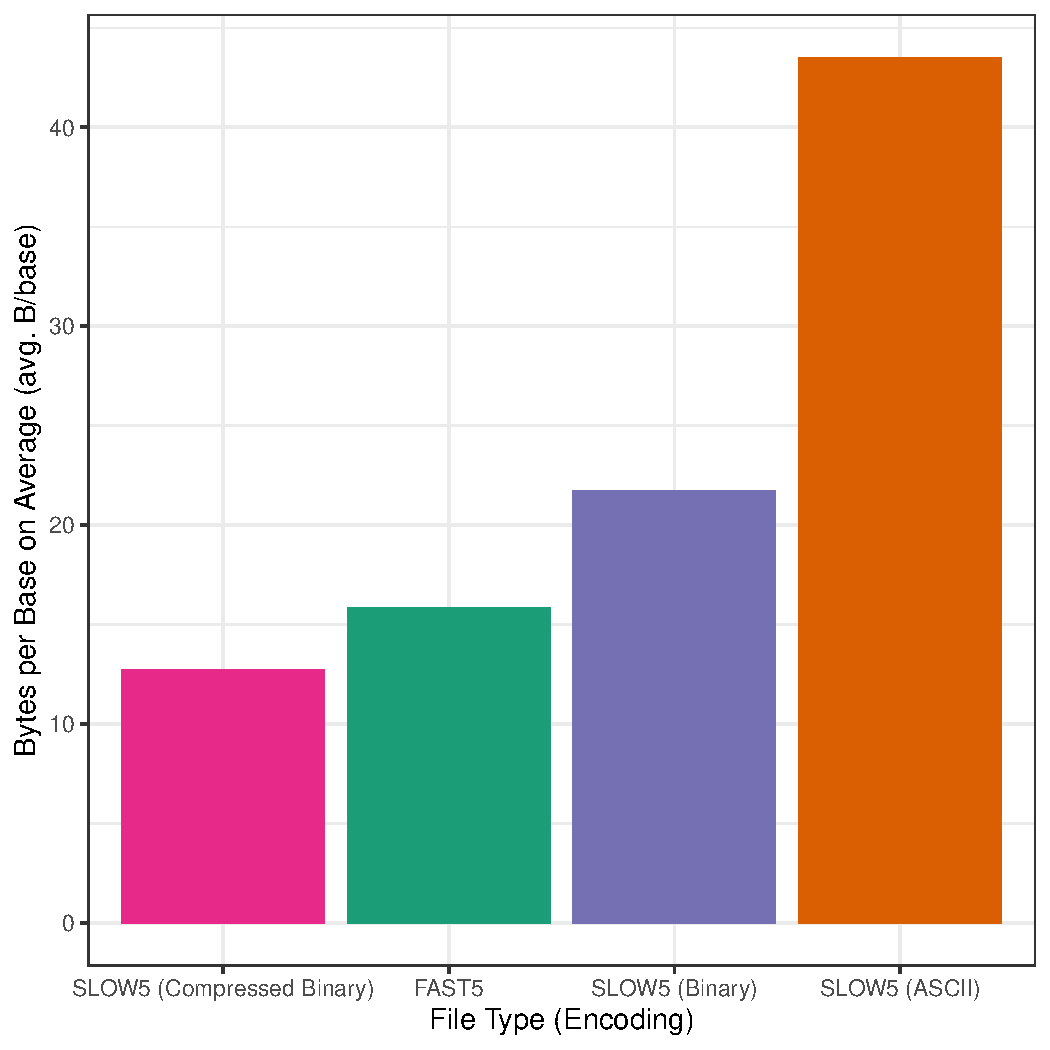
\includegraphics[width=\linewidth]{../../../plot/gpgpu_size.pdf}
    \caption[Bar plot of the bytes stored per base on average for each file type and encoding technique.]{Bar plot of the bytes stored per base on average (avg. B/base) for each file type and encoding technique.}
    \label{fig:size}
\end{figure}

The second experiment's results are displayed in Figure \ref{fig:time}. The line chart graphs the average number of kilobases accessed per second using each file type and encoding over a varying number of threads. It clearly visualises the thread scalability issue (section \ref{sec:back}) of the FAST5 file format (in green) with its read access speed remaining at roughly 2.42 kbases/s on average from 2 to 32 threads. In comparison, the performance of all the SLOW5 file format encodings (in blue, orange and pink) improves with the number of threads used. This relationship appears to be positive, concave-down and non-linear for the server and range of threads used in this experiment.

In particular, the binary encoding of the SLOW5 format (in blue) was found to be the fastest to access for all number of threads, with an access speed of 106.25 kbases/s on average using 32 threads (roughly 44 times faster than using FAST5). The compressed binary and ASCII encodings of the SLOW5 format (in pink and orange) performed in between the binary encoding and FAST5 file format (in blue and green). From 1 to 8 threads, the ASCII encoding (in orange) performed better than the compressed binary encoding (in pink), whilst the relationship reversed between 16 to 32 threads. Using 32 threads, 73.90 kbases/s could be accessed with the compressed binary encoding (in pink), in comparison to 52.63 kbases/s for the ASCII encoding (in orange). In other words, the compressed binary and ASCII encodings of the SLOW5 file format performed 31 and 22 times faster respectively than the FAST5 file format.

\begin{figure}[h]
    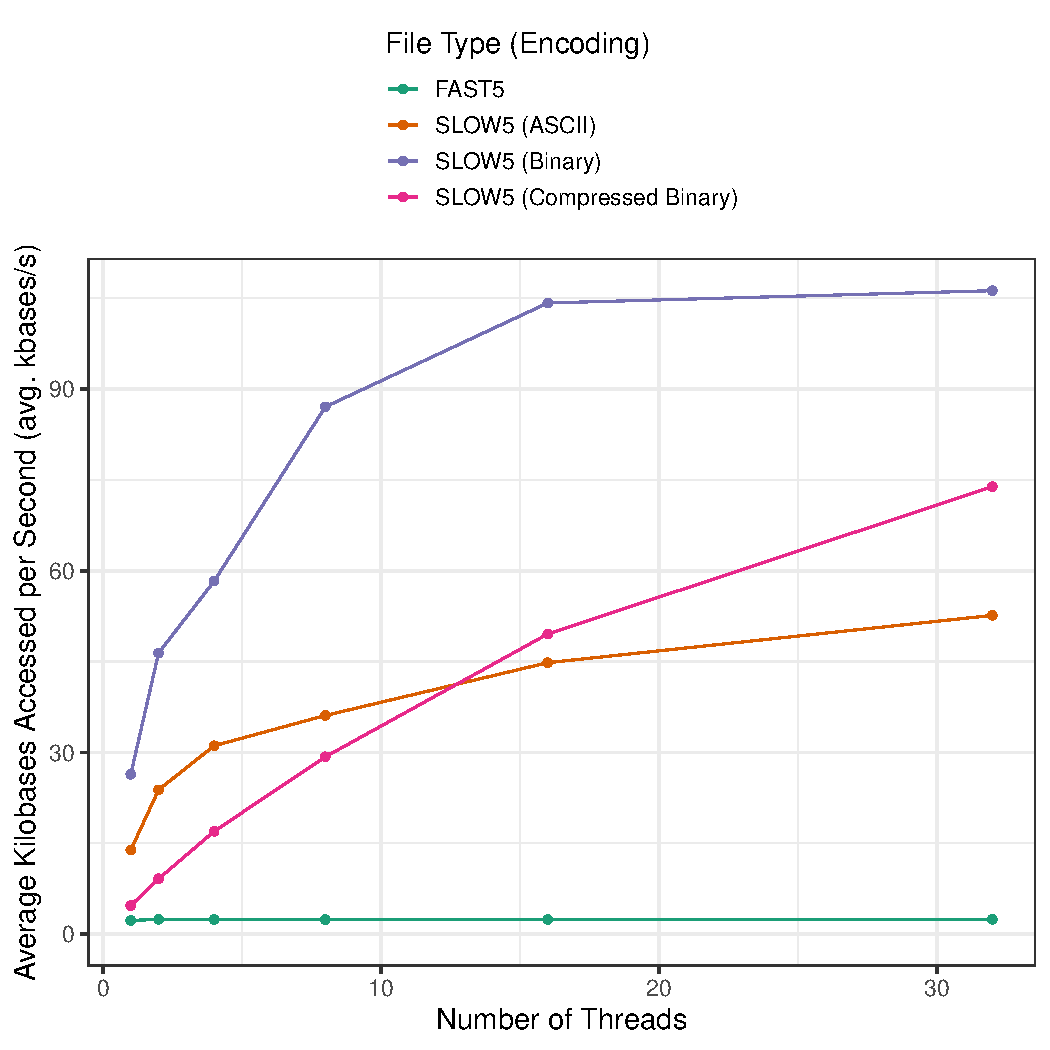
\includegraphics[width=\linewidth]{../../../plot/gpgpu_read_time_thread.pdf}
    \caption[Line chart of the number of kilobases accessed and decoded per second on average for each file format and encoding technique against the number of threads used.]{Line chart of the number of kilobases accessed and decoded per second on average (avg. kbases/s) for each file format and encoding technique against the number of threads used.}
    \label{fig:time}
\end{figure}
